% !TEX root =  master.tex
\section{Bezahlvorgang}
\authorsection{\authorNL}

Wenn der Benutzer all seine Plätze ausgewählt hat und auch die Ermäßigungen angegeben hat, gelangt er zur nächsten Seite, auf der er weitere Daten eingeben muss.

Die Daten werden dabei über \acs{URL}-Parameter weitergegeben.
Dies hat zwar den Nachteil, dass der Benutzer die Werte (z.B. den Gesamtpreis) theoretisch ändern könnte und dann andere Werte angezeigt bekommt.
Dies betrifft jedoch nicht die Sicherheit des Systems, da alle Überprüfung zwangsläufig zumindest im Back-End erfolgen müssen.
Am Beispiel des Preises würde dies bedeuten, dass der Benutzer zwar seine aktuelle Ansicht manipulieren kann, dennoch den korrekten Preis bezahlen muss.

\begin{figure}[ht]
	\centering
	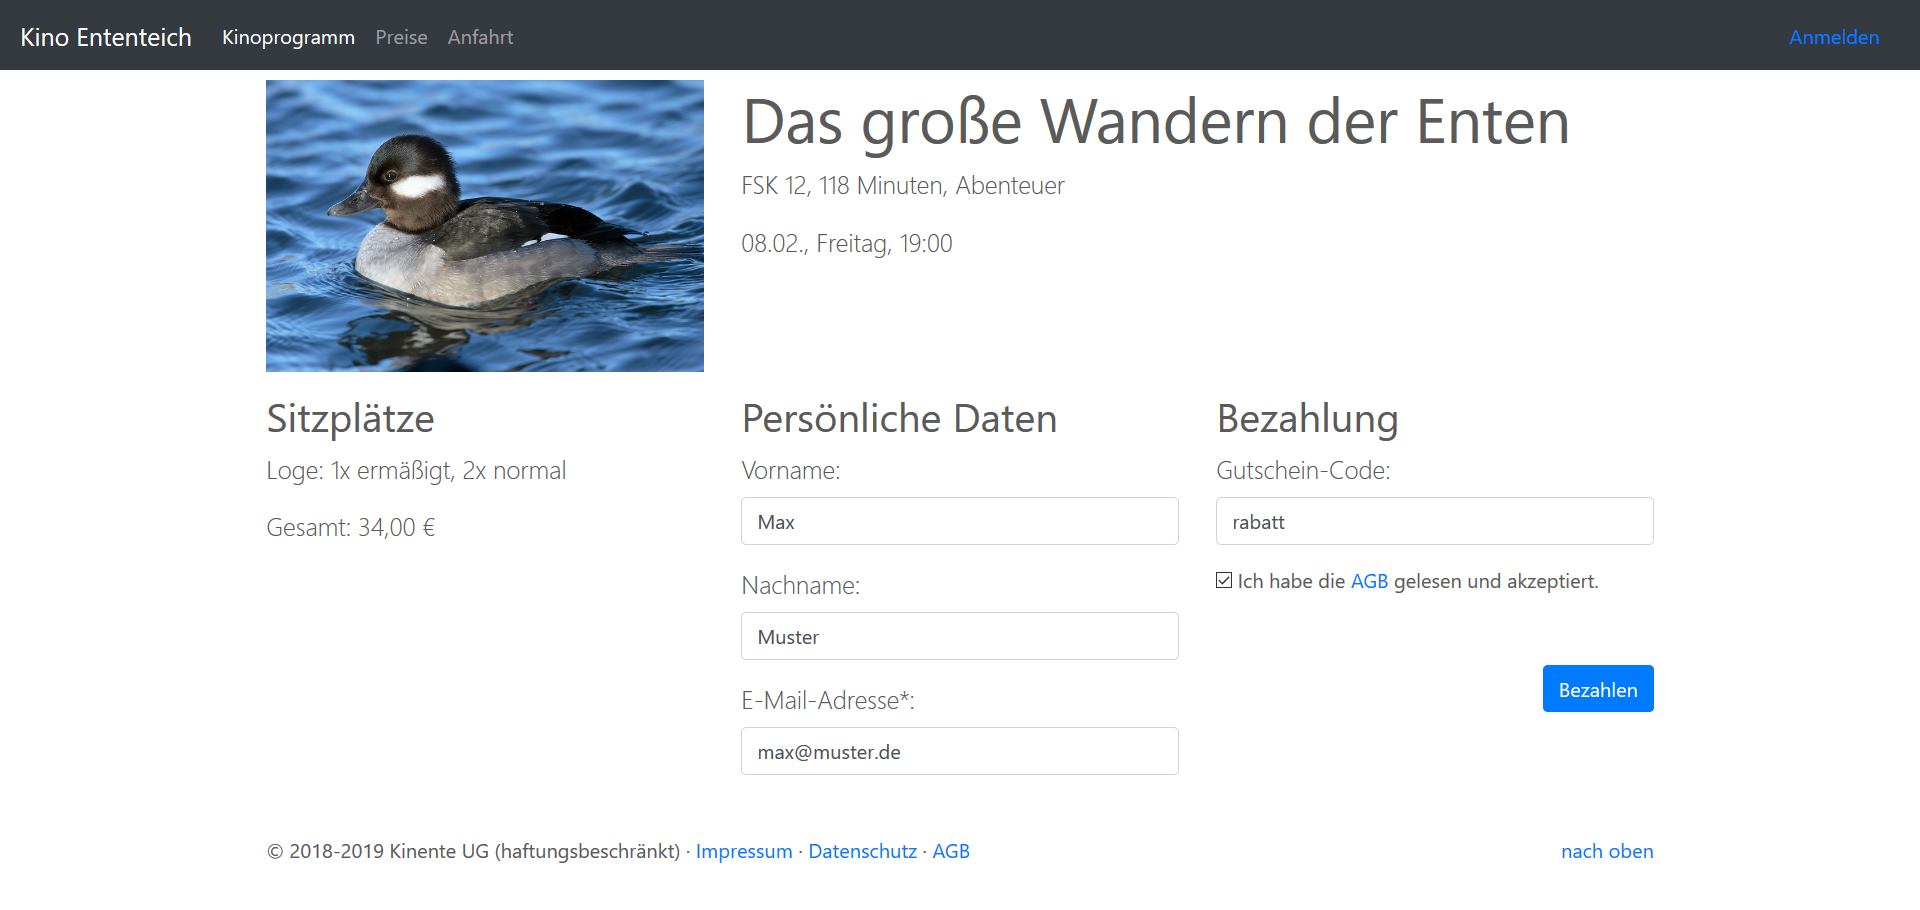
\includegraphics[width=0.98\textwidth]{img/screenshots/vorstellung03}
	\captionsetup{format=hang}
	\caption{Angabe weiterer Daten, die für den Buchungsvorgang relevant sind}
	\label{fig:vorstellung03}
\end{figure}

Im oberen Bereich sieht der Benutzer nochmal allgemeine Informationen zur Vorstellung.
Des Weiteren erhält er eine Zusammenfassung zu seiner Sitzplatzauswahl mit dem Gesamtpreis.
Wenn sich der Benutzer entscheidet, die Sitzplätze verbindlich zu buchen, so wird im Hintergrund eine Nachricht an das Back-End gesendet.

Je nach Antwort wird dann entweder eine Fehlermeldung oder die Bestätigung angezeigt.

Die Bestätigung enthält noch einmal alle Informationen zur Vorstellung, zur Anzahl der Sitzplätze und zum gezahlten Kaufpreis.
Unter einer kurzen Beschreibung zum weiteren Verlauf findet der Benutzer sein Ticket in Form eines \acs{QR-Code}s.
In diesem ist ein eindeutiger Verweis auf die Reservierung und somit auf alle Tickets gespeichert.
Der \acs{QR-Code} wird dabei unter Zuhilfenahme einer quelloffenen Bibliothek\footnote{\url{https://github.com/nayuki/QR-Code-generator}} erzeugt.

\begin{figure}[ht]
	\centering
	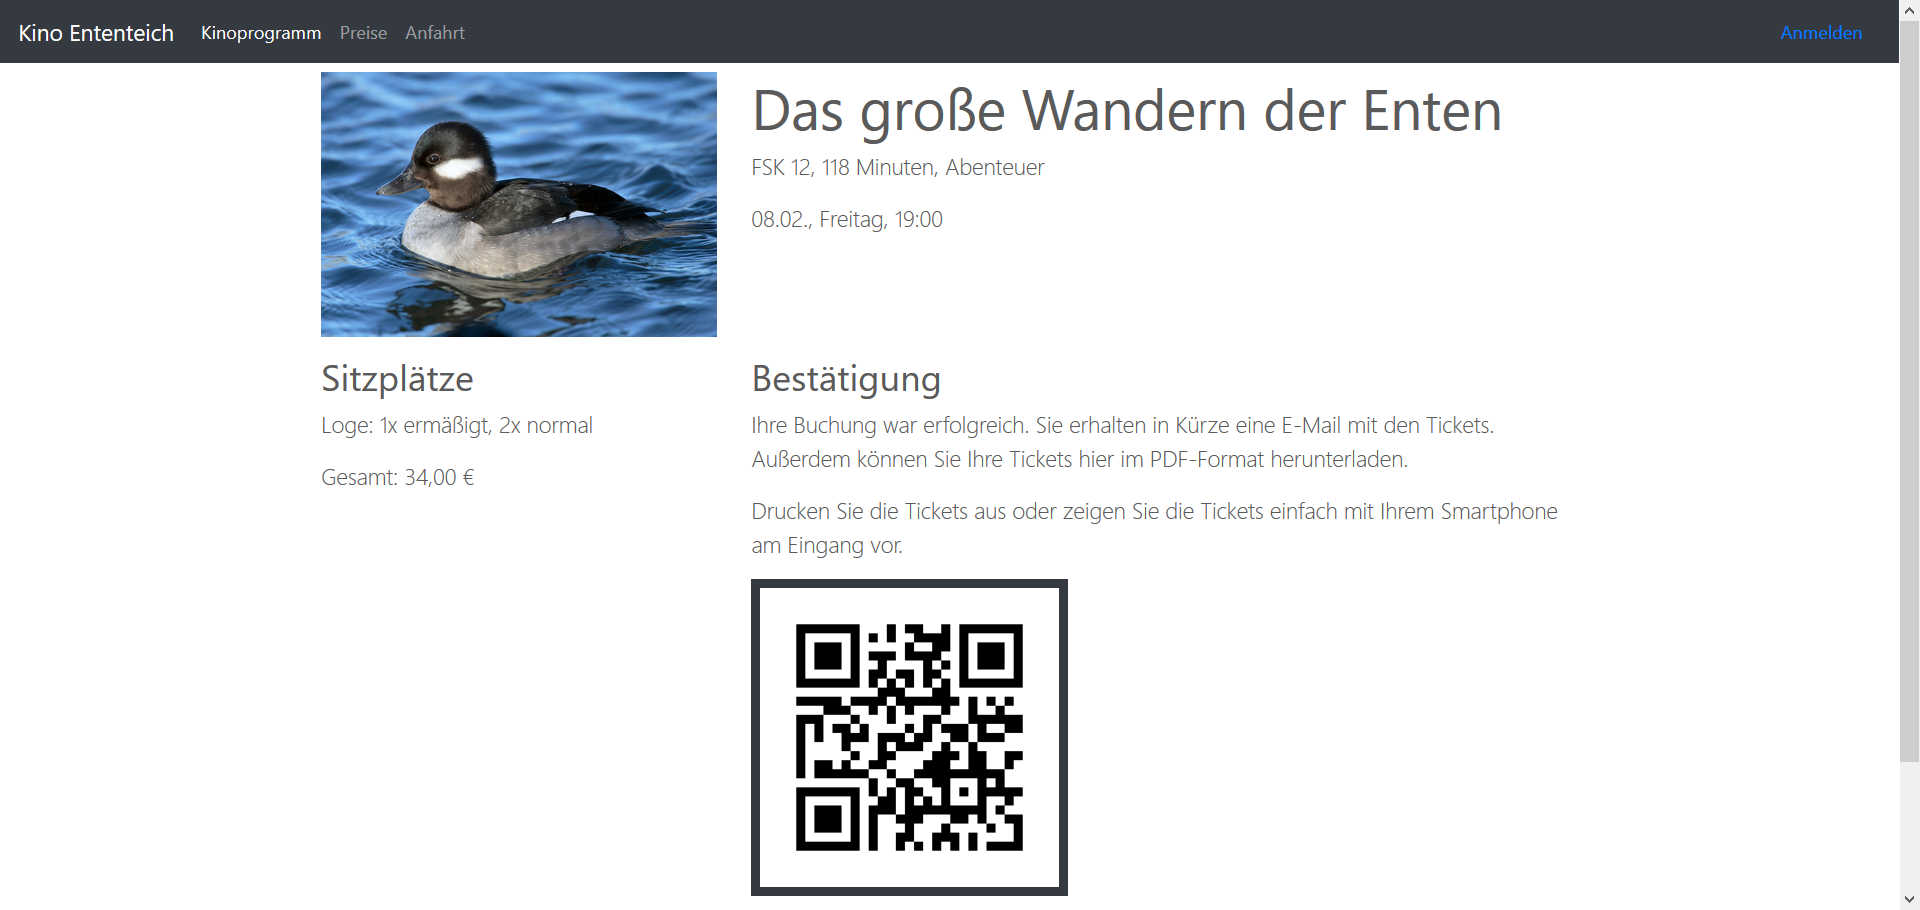
\includegraphics[width=0.98\textwidth]{img/screenshots/vorstellung04}
	\captionsetup{format=hang}
	\caption{Bestätigung einer Reservierung und Anzeige des \acs{QR-Code}s}
	\label{fig:vorstellung04}
\end{figure}